% Options for packages loaded elsewhere
\PassOptionsToPackage{unicode}{hyperref}
\PassOptionsToPackage{hyphens}{url}
%
\documentclass[
]{article}
\usepackage{amsmath,amssymb}
\usepackage{lmodern}
\usepackage{iftex}
\ifPDFTeX
  \usepackage[T1]{fontenc}
  \usepackage[utf8]{inputenc}
  \usepackage{textcomp} % provide euro and other symbols
\else % if luatex or xetex
  \usepackage{unicode-math}
  \defaultfontfeatures{Scale=MatchLowercase}
  \defaultfontfeatures[\rmfamily]{Ligatures=TeX,Scale=1}
\fi
% Use upquote if available, for straight quotes in verbatim environments
\IfFileExists{upquote.sty}{\usepackage{upquote}}{}
\IfFileExists{microtype.sty}{% use microtype if available
  \usepackage[]{microtype}
  \UseMicrotypeSet[protrusion]{basicmath} % disable protrusion for tt fonts
}{}
\makeatletter
\@ifundefined{KOMAClassName}{% if non-KOMA class
  \IfFileExists{parskip.sty}{%
    \usepackage{parskip}
  }{% else
    \setlength{\parindent}{0pt}
    \setlength{\parskip}{6pt plus 2pt minus 1pt}}
}{% if KOMA class
  \KOMAoptions{parskip=half}}
\makeatother
\usepackage{xcolor}
\usepackage[margin=1in]{geometry}
\usepackage{color}
\usepackage{fancyvrb}
\newcommand{\VerbBar}{|}
\newcommand{\VERB}{\Verb[commandchars=\\\{\}]}
\DefineVerbatimEnvironment{Highlighting}{Verbatim}{commandchars=\\\{\}}
% Add ',fontsize=\small' for more characters per line
\usepackage{framed}
\definecolor{shadecolor}{RGB}{248,248,248}
\newenvironment{Shaded}{\begin{snugshade}}{\end{snugshade}}
\newcommand{\AlertTok}[1]{\textcolor[rgb]{0.94,0.16,0.16}{#1}}
\newcommand{\AnnotationTok}[1]{\textcolor[rgb]{0.56,0.35,0.01}{\textbf{\textit{#1}}}}
\newcommand{\AttributeTok}[1]{\textcolor[rgb]{0.77,0.63,0.00}{#1}}
\newcommand{\BaseNTok}[1]{\textcolor[rgb]{0.00,0.00,0.81}{#1}}
\newcommand{\BuiltInTok}[1]{#1}
\newcommand{\CharTok}[1]{\textcolor[rgb]{0.31,0.60,0.02}{#1}}
\newcommand{\CommentTok}[1]{\textcolor[rgb]{0.56,0.35,0.01}{\textit{#1}}}
\newcommand{\CommentVarTok}[1]{\textcolor[rgb]{0.56,0.35,0.01}{\textbf{\textit{#1}}}}
\newcommand{\ConstantTok}[1]{\textcolor[rgb]{0.00,0.00,0.00}{#1}}
\newcommand{\ControlFlowTok}[1]{\textcolor[rgb]{0.13,0.29,0.53}{\textbf{#1}}}
\newcommand{\DataTypeTok}[1]{\textcolor[rgb]{0.13,0.29,0.53}{#1}}
\newcommand{\DecValTok}[1]{\textcolor[rgb]{0.00,0.00,0.81}{#1}}
\newcommand{\DocumentationTok}[1]{\textcolor[rgb]{0.56,0.35,0.01}{\textbf{\textit{#1}}}}
\newcommand{\ErrorTok}[1]{\textcolor[rgb]{0.64,0.00,0.00}{\textbf{#1}}}
\newcommand{\ExtensionTok}[1]{#1}
\newcommand{\FloatTok}[1]{\textcolor[rgb]{0.00,0.00,0.81}{#1}}
\newcommand{\FunctionTok}[1]{\textcolor[rgb]{0.00,0.00,0.00}{#1}}
\newcommand{\ImportTok}[1]{#1}
\newcommand{\InformationTok}[1]{\textcolor[rgb]{0.56,0.35,0.01}{\textbf{\textit{#1}}}}
\newcommand{\KeywordTok}[1]{\textcolor[rgb]{0.13,0.29,0.53}{\textbf{#1}}}
\newcommand{\NormalTok}[1]{#1}
\newcommand{\OperatorTok}[1]{\textcolor[rgb]{0.81,0.36,0.00}{\textbf{#1}}}
\newcommand{\OtherTok}[1]{\textcolor[rgb]{0.56,0.35,0.01}{#1}}
\newcommand{\PreprocessorTok}[1]{\textcolor[rgb]{0.56,0.35,0.01}{\textit{#1}}}
\newcommand{\RegionMarkerTok}[1]{#1}
\newcommand{\SpecialCharTok}[1]{\textcolor[rgb]{0.00,0.00,0.00}{#1}}
\newcommand{\SpecialStringTok}[1]{\textcolor[rgb]{0.31,0.60,0.02}{#1}}
\newcommand{\StringTok}[1]{\textcolor[rgb]{0.31,0.60,0.02}{#1}}
\newcommand{\VariableTok}[1]{\textcolor[rgb]{0.00,0.00,0.00}{#1}}
\newcommand{\VerbatimStringTok}[1]{\textcolor[rgb]{0.31,0.60,0.02}{#1}}
\newcommand{\WarningTok}[1]{\textcolor[rgb]{0.56,0.35,0.01}{\textbf{\textit{#1}}}}
\usepackage{graphicx}
\makeatletter
\def\maxwidth{\ifdim\Gin@nat@width>\linewidth\linewidth\else\Gin@nat@width\fi}
\def\maxheight{\ifdim\Gin@nat@height>\textheight\textheight\else\Gin@nat@height\fi}
\makeatother
% Scale images if necessary, so that they will not overflow the page
% margins by default, and it is still possible to overwrite the defaults
% using explicit options in \includegraphics[width, height, ...]{}
\setkeys{Gin}{width=\maxwidth,height=\maxheight,keepaspectratio}
% Set default figure placement to htbp
\makeatletter
\def\fps@figure{htbp}
\makeatother
\setlength{\emergencystretch}{3em} % prevent overfull lines
\providecommand{\tightlist}{%
  \setlength{\itemsep}{0pt}\setlength{\parskip}{0pt}}
\setcounter{secnumdepth}{-\maxdimen} % remove section numbering
\ifLuaTeX
  \usepackage{selnolig}  % disable illegal ligatures
\fi
\IfFileExists{bookmark.sty}{\usepackage{bookmark}}{\usepackage{hyperref}}
\IfFileExists{xurl.sty}{\usepackage{xurl}}{} % add URL line breaks if available
\urlstyle{same} % disable monospaced font for URLs
\hypersetup{
  pdftitle={Exercises: RMarkdown},
  hidelinks,
  pdfcreator={LaTeX via pandoc}}

\title{Exercises: RMarkdown}
\author{}
\date{\vspace{-2.5em}}

\begin{document}
\maketitle

\hypertarget{exercises-rmarkdown}{%
\section{Exercises: RMarkdown}\label{exercises-rmarkdown}}

In this practical we will introduce the basics of using RMarkdown and
some of its features.

\hypertarget{introduction}{%
\subsection{Introduction}\label{introduction}}

R Markdown is a file format for making dynamic documents with R. An R
Markdown document is written in markdown (an easy-to-write plain text
format) and contains \emph{chunks} of embedded R code.

An RMarkdown document is rendered by \emph{knitting} the file.

The \texttt{rmarkdown} package will call the \texttt{knitr} package.
\texttt{knitr} will run each chunk of R code in the document and append
the results of the code to the document next to the code chunk. This
workflow saves time and facilitates reproducible reports.

Consider how authors typically include graphs (or tables, or numbers) in
a report. The author makes the graph, saves it as a file, and then copy
and pastes it into the final report. This process relies on manual
labour. If the data changes, the author must repeat the entire process
to update the graph.

In the R Markdown paradigm, each report contains the code it needs to
make its own graphs, tables, numbers, etc. The author can automatically
update the report by re-knitting.

\hypertarget{creating-a-r-markdown-document}{%
\subsection{Creating a R Markdown
document}\label{creating-a-r-markdown-document}}

To create an R Markdown report, open a plain text file and save it with
the extension \emph{.Rmd}. You can open a plain text file in your
scripts editor by clicking \emph{File \textgreater{} New File
\textgreater{} Text File} in the RStudio tool bar, or using the
\emph{Wizard} by selecting \emph{File \textgreater{} New File
\textgreater{} R Markdown \ldots{}}

\hypertarget{rendering}{%
\paragraph{Rendering}\label{rendering}}

To go from R Markdown to pdf or html you can click on the \emph{Knit}
icon thats above the file in the scripts editor. A drop down menu will
let you select the type of output that you want. RStudio will show you a
preview of the new output and save the output file in your working
directory. You can manually render an R Markdown file with
\texttt{rmarkdown::render()}.

\hypertarget{text-formatting}{%
\subsection{Text formatting}\label{text-formatting}}

Markdown is designed to be easy to read and easy to write. It is also
very easy to learn.

Go to the drop down menu and select \emph{Help \textgreater{} Markdown
Quck Reference}. This will open a cheat sheet in the Help pane.

\hypertarget{code-chunks}{%
\subsection{Code chunks}\label{code-chunks}}

To run code inside an R Markdown document, you need to insert a chunk.
There are three ways to do so:

\begin{itemize}
\item
  The keyboard shortcut Cmd/Ctrl + Alt + I
\item
  The \emph{Insert} button icon in the editor tool bar
\item
  By manually typing the chunk delimiters \texttt{\{r\}\ and}.
\end{itemize}

Think of a chunk like a function. A chunk should be relatively
self-contained, and focussed around a single task.

\hypertarget{chunk-names}{%
\subsubsection{Chunk names}\label{chunk-names}}

Chunks can be given an optional name: ```\{r by-name\}. This has three
advantages:

\begin{itemize}
\item
  You can more easily navigate to specific chunks using the drop-down
  code navigator in the bottom-left of the script editor:
\item
  Graphics produced by the chunks will have useful names that make them
  easier to use elsewhere. More on that in other important options.
\item
  You can set up networks of cached chunks to avoid re-performing
  expensive computations on every run.
\end{itemize}

\hypertarget{chunk-options}{%
\subsubsection{Chunk options}\label{chunk-options}}

Chunk output can be customised. A full list is here
\url{http://yihui.name/knitr/options/}.

The most important set of options controls if your code block is
executed and what results are inserted in the finished report:

\begin{itemize}
\item
  \texttt{eval\ =\ FALSE} prevents code from being evaluated. (And
  obviously if the code is not run, no results will be generated). This
  is useful for displaying example code, or for disabling a large block
  of code without commenting each line.
\item
  \texttt{include\ =\ FALSE} runs the code, but doesn't show the code or
  results in the final document. Use this for setup code that you don't
  want cluttering your report.
\item
  \texttt{echo\ =\ FALSE} prevents code, but not the results from
  appearing in the finished file. Use this when writing reports aimed at
  people who don't want to see the underlying R code.
\item
  \texttt{message\ =\ FALSE} or \texttt{warning\ =\ FALSE} prevents
  messages or warnings from appearing in the finished file.
\item
  \texttt{results\ =\ \textquotesingle{}hide\textquotesingle{}} hides
  printed output;
  \texttt{fig.show\ =\ \textquotesingle{}hide\textquotesingle{}} hides
  plots.
\item
  \texttt{error\ =\ TRUE} causes the render to continue even if code
  returns an error. This is rarely something you'll want to include in
  the final version of your report, but can be very useful if you need
  to debug exactly what is going on inside your .Rmd. It's also useful
  if you're teaching R and want to deliberately include an error. The
  default, error = FALSE causes knitting to fail if there is a single
  error in the document.
\end{itemize}

\hypertarget{tables-in-r-markdown}{%
\subsection{Tables in R Markdown}\label{tables-in-r-markdown}}

By default, R Markdown prints data frames and matrices as you'd see them
in the console. If you prefer that data be displayed with additional
formatting you can use the \texttt{knitr::kable} function. For even
deeper customisation, consider the \texttt{xtable}, \texttt{stargazer},
\texttt{pander}, \texttt{tables}, and \texttt{ascii} packages

\hypertarget{inline-code}{%
\subsection{Inline code}\label{inline-code}}

To embed R code in a line of text, surround the code with a pair of back
ticks and the letter r, like this.

\begin{Shaded}
\begin{Highlighting}[]
\StringTok{\textasciigrave{}}\AttributeTok{r  ICER is 200/0.5}\StringTok{\textasciigrave{}}
\end{Highlighting}
\end{Shaded}

knitr will replace the inline code with its result in your final
document (inline code is always replaced by its result). The result will
appear as if it were part of the original text

\hypertarget{yaml-header}{%
\subsection{YAML header}\label{yaml-header}}

A YAML header to control how rmarkdown renders your \emph{.Rmd} file. A
YAML header is a section of key: value pairs surrounded by --- marks.

The \texttt{output:} value determines what type of output to convert the
file into when you call \texttt{rmarkdown::render()}.

\texttt{output:} recognizes the following values:

\begin{itemize}
\tightlist
\item
  \texttt{html\_document}, which will create HTML output (default)
\item
  \texttt{pdf\_document}, which will create PDF output
\item
  \texttt{word\_document}, which will create Word output
\end{itemize}

If you use the RStudio IDE knit button to render your file, the
selection you make in the gui will override the output: setting.

\hypertarget{putting-it-all-together-in-an-example-report}{%
\subsection{Putting it all together in an example
report}\label{putting-it-all-together-in-an-example-report}}

\begin{itemize}
\item
  Create a new R Markdown document with main sections with headings
  Introduction, Data, Methods, Results and Conclusions.
\item
  Include some subheadings like Model Fitting and Recommendations, say.
\item
  In the Conclusions make numbered list of the main findings.
\item
  Include a link to the Briggs papers on which the original
  cost-effectiveness analysis is based i.e. \emph{An Introduction to
  Markov Modelling for Economic Evaluation, Andrew Briggs and Mark
  Sculpher}
\item
  Change the date of the document so that it will always be today's date
  using the following
\end{itemize}

\begin{Shaded}
\begin{Highlighting}[]
\NormalTok{date}\SpecialCharTok{:} \StringTok{"\textasciigrave{}r format(Sys.time(), \textquotesingle{}\%d \%B, \%Y\textquotesingle{})\textasciigrave{}"}
\end{Highlighting}
\end{Shaded}

Pick a date format that you prefer

\begin{itemize}
\tightlist
\item
  Include the plot created with the following code
\end{itemize}

\begin{Shaded}
\begin{Highlighting}[]
\FunctionTok{plot}\NormalTok{(}\DecValTok{10}\NormalTok{, }\FloatTok{0.1}\NormalTok{,}
     \AttributeTok{xlab =} \StringTok{"Incremental QALYs"}\NormalTok{,}
     \AttributeTok{ylab =} \StringTok{"Incremental costs"}\NormalTok{,}
     \AttributeTok{xlim =} \FunctionTok{c}\NormalTok{(}\SpecialCharTok{{-}}\DecValTok{1}\NormalTok{, }\DecValTok{12}\NormalTok{),}
     \AttributeTok{ylim =} \FunctionTok{c}\NormalTok{(}\SpecialCharTok{{-}}\FloatTok{0.1}\NormalTok{, }\FloatTok{0.2}\NormalTok{),}
     \AttributeTok{pch =} \DecValTok{20}\NormalTok{)}
\FunctionTok{abline}\NormalTok{(}\AttributeTok{a =} \DecValTok{0}\NormalTok{, }\AttributeTok{b =} \FloatTok{0.02}\NormalTok{)}
\end{Highlighting}
\end{Shaded}

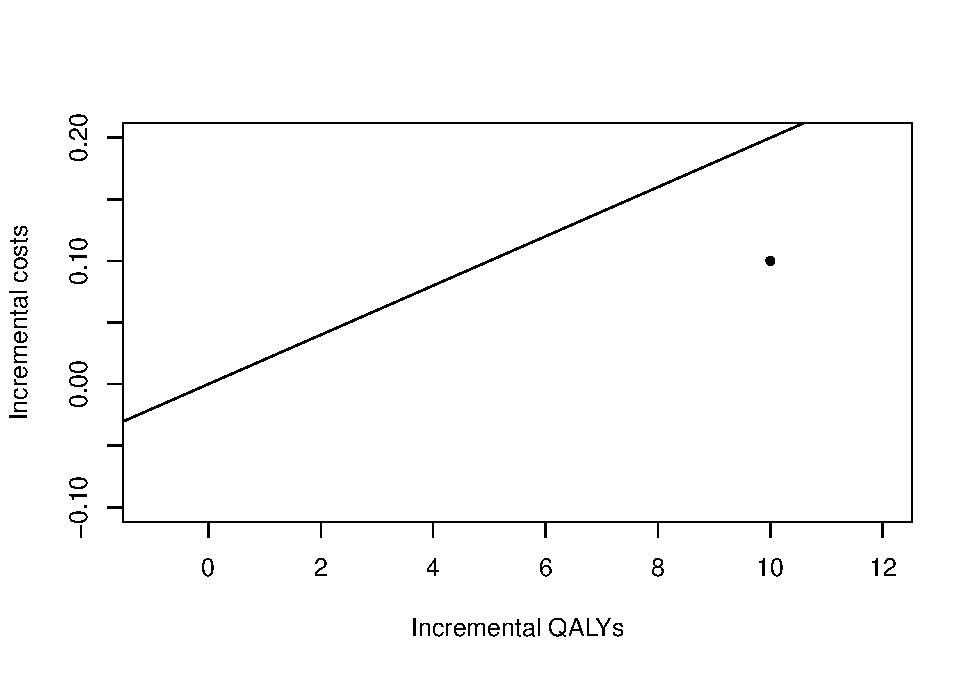
\includegraphics{literate-programming-exercises_files/figure-latex/ceplane-1.pdf}

\begin{itemize}
\item
  Resize this plot using the chunk options
\item
  Create a table that shows the cost and QALYs for two interventions and
  their incremental values and ICER. Here something to start with.
\end{itemize}

\begin{Shaded}
\begin{Highlighting}[]
\NormalTok{intervention }\SpecialCharTok{|}\NormalTok{ cost }\SpecialCharTok{|}\NormalTok{ QALY }\SpecialCharTok{|}\NormalTok{ delta c }\SpecialCharTok{|}\NormalTok{ delta QALY }\SpecialCharTok{|}\NormalTok{ ICER}
\SpecialCharTok{{-}{-}{-}{-}{-}{-}{-}{-}{-}{-}{-}{-}{-}}\ErrorTok{|}\SpecialCharTok{{-}{-}{-}{-}{-}{-}}\ErrorTok{|}\SpecialCharTok{{-}{-}{-}{-}{-}{-}}\ErrorTok{|}\SpecialCharTok{{-}{-}{-}{-}{-}{-}{-}{-}{-}}\ErrorTok{|}\SpecialCharTok{{-}{-}{-}{-}{-}{-}{-}{-}{-}{-}{-}{-}}\ErrorTok{|}\SpecialCharTok{{-}{-}{-}{-}{-}}
\NormalTok{drug a       }\SpecialCharTok{|} \DecValTok{100}  \SpecialCharTok{|} \FloatTok{0.5}  \SpecialCharTok{|}         \ErrorTok{|}            \ErrorTok{|}
\SpecialCharTok{{-}{-}{-}{-}{-}{-}{-}{-}{-}{-}{-}{-}{-}}\ErrorTok{|}\SpecialCharTok{{-}{-}{-}{-}{-}{-}}\ErrorTok{|}\SpecialCharTok{{-}{-}{-}{-}{-}{-}}\ErrorTok{|}\SpecialCharTok{{-}{-}{-}{-}{-}{-}{-}{-}{-}}\ErrorTok{|}\SpecialCharTok{{-}{-}{-}{-}{-}{-}{-}{-}{-}{-}{-}{-}}\ErrorTok{|}\SpecialCharTok{{-}{-}{-}{-}{-}}
\NormalTok{drug b       }\SpecialCharTok{|} \DecValTok{50}   \SpecialCharTok{|} \FloatTok{0.1}  \SpecialCharTok{|}  \DecValTok{50}     \SpecialCharTok{|}  \FloatTok{0.4}       \SpecialCharTok{|} \DecValTok{20}
\end{Highlighting}
\end{Shaded}

\begin{itemize}
\tightlist
\item
  Now create the same table but do this programmatically. That is create
  a data frame with the entries and then use \texttt{knitr::kable} to
  convert to markdown.
\end{itemize}

Here's an example template to get you started

\begin{Shaded}
\begin{Highlighting}[]
\FunctionTok{data.frame}\NormalTok{(}\AttributeTok{intervention =} \FunctionTok{c}\NormalTok{(}\StringTok{"drug a"}\NormalTok{, }\StringTok{"drug b"}\NormalTok{),}
           \AttributeTok{cost =} \FunctionTok{c}\NormalTok{(}\DecValTok{100}\NormalTok{,}\DecValTok{50}\NormalTok{),}
           \AttributeTok{QALY =} \FunctionTok{c}\NormalTok{(}\FloatTok{0.5}\NormalTok{,}\FloatTok{0.1}\NormalTok{),}
           \AttributeTok{delta\_c =} \FunctionTok{c}\NormalTok{(}\ConstantTok{NA}\NormalTok{, }\DecValTok{50}\NormalTok{),}
           \AttributeTok{delta\_QALY =} \FunctionTok{c}\NormalTok{(}\ConstantTok{NA}\NormalTok{, }\FloatTok{0.4}\NormalTok{),}
           \AttributeTok{ICER =} \FunctionTok{c}\NormalTok{(}\ConstantTok{NA}\NormalTok{, }\DecValTok{20}\NormalTok{))}\SpecialCharTok{|\textgreater{}} 
\NormalTok{knitr}\SpecialCharTok{::}\FunctionTok{kable}\NormalTok{()}
\end{Highlighting}
\end{Shaded}


\end{document}
